\documentclass{article}
\usepackage{blindtext}
\usepackage[margin=1in]{geometry}
\usepackage[utf8]{inputenc}
\usepackage{amsmath}
\usepackage{stackengine}
\usepackage[pdftex]{graphicx}
\usepackage{float}
\usepackage{newlfont}
\usepackage{amssymb}
\usepackage{verbatim} 
\usepackage{subcaption}
\usepackage[final]{pdfpages}
\usepackage{setspace}
\usepackage{bbm}
\setlength{\parindent}{0pt}

\title{Predicting Soccer Matches with Bradley-Terry Models and Extensions}
\author{Sanjay Hariharan and Ilan Man}
\date{\today} 
\begin{document}
\maketitle

\section{Problem Motivation}

Predicting the outcome of competitions is a well-studied and desirable subject, for both gamblers and sports fans alike. Given a Kaggle dataset of competing European Soccer teams, we set out to build a predictive model that can correctly predict the winner of head-to-head matchups. \textbf{INSERT SOMETHING ABOUT DATASET DIMENSIONS LIKE YOU HAD BEFORE, I.E NUMBER OF TEAMS, AVERAGE NUMBER OF MATCHES PLAYED, MAYBE NUMBER OF LEAGURES? JUST TO GET A SENSE OF THE SIZE OF THE DATASET.}
The dataset contains match level results and team specific attributes over eight years. Using the dataset we intend to understand the relative strength of teams using a Bradley-Terry model. 

\section{Exploratory Data Analysis}

We perform a myriad of exploratory analyses to better understand the variables' distributions and to provoke further questions to explore. For example, below we plotted goals scored (both by count and proportion) for home teams verses away for a random subset of teams. \\

\begin{figure}[H]
\centering
\begin{subfigure}{.5\textwidth}
  \centering
  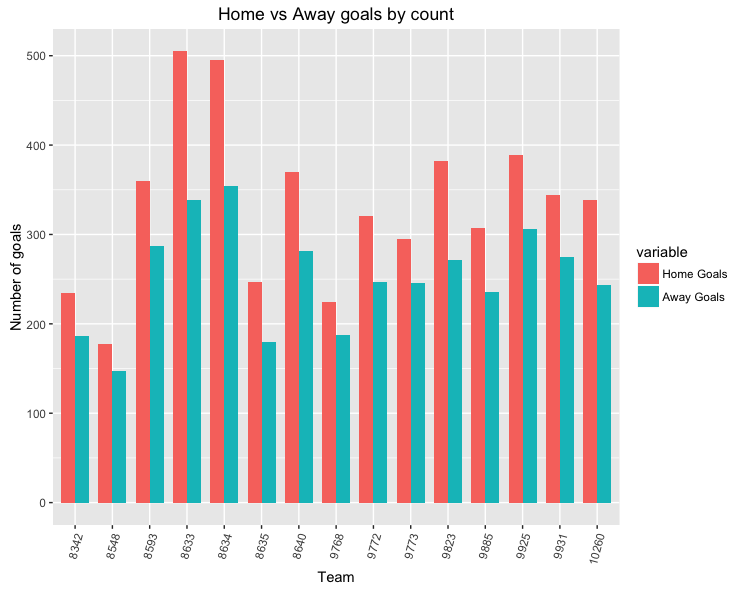
\includegraphics[width=.8\linewidth]{figures/homevsawaycount.png}
  \caption{Count of Goals scored}
  \label{fig:sub1}
\end{subfigure}%
\begin{subfigure}{.5\textwidth}
  \centering
  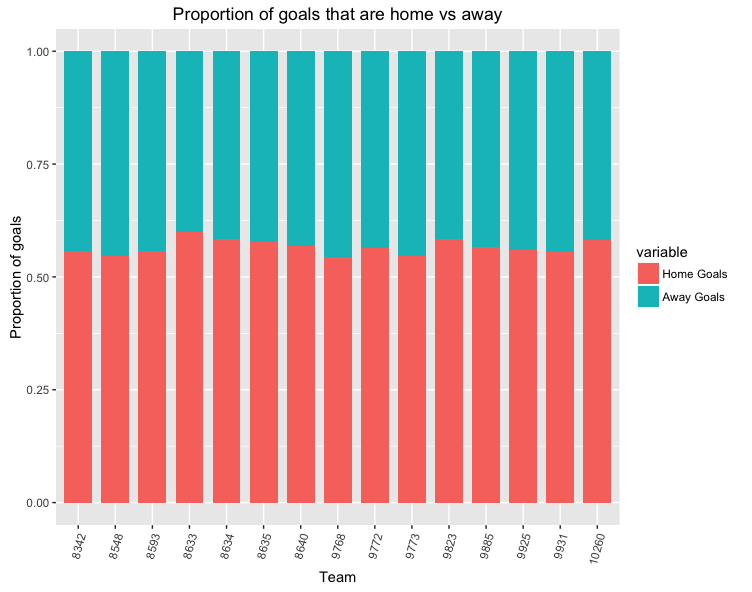
\includegraphics[width=.8\linewidth]{figures/homevsawaygoals.png}
  \caption{Proportion of Goals scored}
  \label{fig:sub2}
\end{subfigure}
\end{figure}

From the plots above, we can see that these teams average a greater number and proportion of goals scored at home than away. This confirms our intuition that home field does confer an advantage in matches. In addition, bookies generally favor a home team at 53\%, so we consider a model-based approach which includes a home vs away covariate.\\

As indicated above, the dataset also contains attributes specific to each team. In particular, FIFA provides a score on a variety of measures including defense, passing, shooting, and build up speed. Intuitively, all else equal, teams with higher ratings are more likely to win matches. \\

\begin{figure}[H]
\centering
\begin{subfigure}{.5\textwidth}
  \centering
  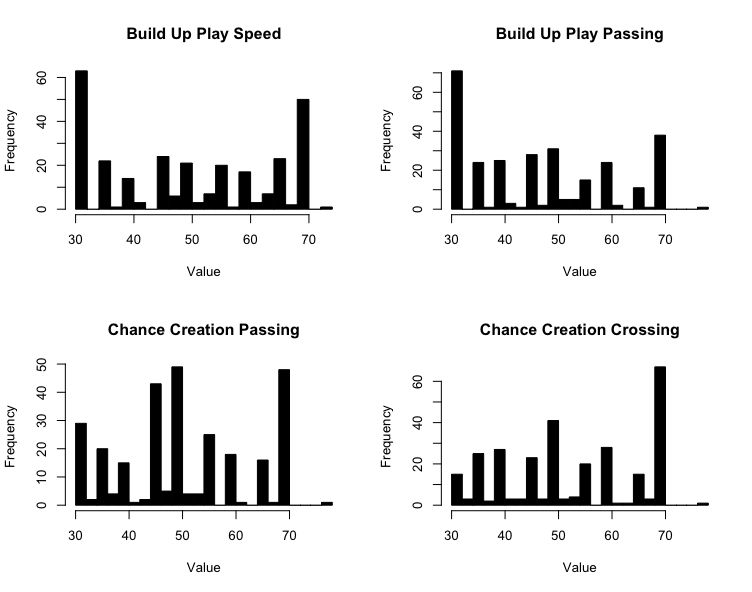
\includegraphics[width=.8\linewidth]{figures/hist1.png}
  \label{fig:sub1}
\end{subfigure}%
\begin{subfigure}{.5\textwidth}
  \centering
  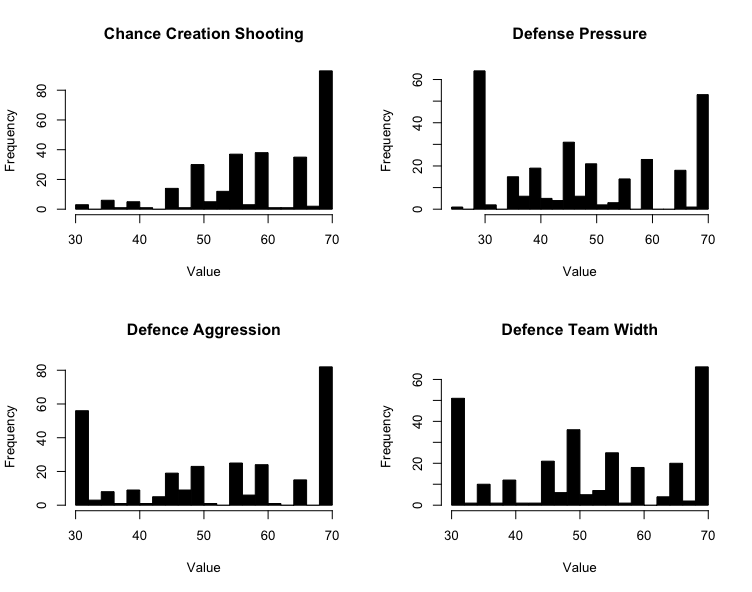
\includegraphics[width=.8\linewidth]{figures/hist2.png}
  \label{fig:sub2}
\end{subfigure}
\end{figure}

The histograms above show no discernible pattern, except for minor bimodality for some measures, such as defense aggression and build-up play speed. This indicates that there may be a strong divide among high rated and low rated teams for some measures. In order to build a richer model, we consider including team attributes as a predictor of winning or losing a match.\\

Our analysis above prompted the following questions that we seek to answer in our paper:

\begin{itemize}
	\item What is the relative strength of one team compared to another?
	\item Does playing at home offer a significant advantage?
	\item Which team attributes contribute most significantly to winning a match?
\end{itemize}

\section{Modeling}

Our main goal is to predict the outcome of any head-to-head soccer game. As such, the ability to estimate the probability of a pairwise matchup is desireable. The canonical Bradley-Terry model is flexible, interpretable, and provides us with the inference necessary to achieve this goal. Later we consider extensions to the basic model, studying home team effect and team-specific predictors. \textbf{SHOULD WE MAKE A NOTE THAT TEAMS HAVE DIFFERENT OPPONENTS, SO NOT EVERY TEAM PLAYS EACH OTHER. AND SINCE THE LEVEL OF OPPONENTS VARY, ITS NOT CLEAR  (TO ME ANYWAY) IF OPPONENT STRENGTH CAN BE CONTROLLED FOR IN THESE MODELS. IF NOT, WE SHOULD NOTE IT BECAUSE ITS IMPORTANT. OR WE MENTION IT IN THE LIMITATIONS/EXTENSIONS SECTION}

\subsection{Standard Bradley-Terry Model}

The standard Bradley-Terry model does not take into account any covariate effects. It is simply the head-to-head matchups along with the winner. The model can be expressed in the logit-linear form, for teams $i$ and $j$:

$$\text{logit}[P(i > j)] = \lambda_i - \lambda_j$$

$\lambda_i$ here is the coefficient estimate for team $i$. There are 2 ways to interpret the model output:

\begin{enumerate}
	\item $\lambda_i$ represents team $i$'s relative strength compared with other team's
	\item $\lambda_i - \lambda_j$ represents the log-odds of Team $i$ beating Team $j$ in any given match up
\end{enumerate}

\subsubsection{Results}

We present the model outcome for the 3 teams with the best and worst winning percentage:

\begin{table}[H]
\centering
\begin{tabular}{|r|rrrr|}
  \hline
 & Team Name & Win \% & $\hat{\lambda_i}$ & SE($\hat{\lambda_i}$) \\ 
  \hline
   &  FC Barcelona & 0.769 & 2.792 & 0.299 \\ 
 Best  &  Real Madrid CF & 0.750 & 2.385 & 0.280 \\ 
   &  SL Benfica & 0.745 & 3.079 & 0.497 \\ \cline{1-5}
   &  Cordoba CF & 0.079 & -1.482 & 0.660 \\ 
Worst   &  SpVgg Greuther Furth & 0.118 & -1.586  & 0.577 \\ 
   & FC Dordrecht & 0.118 & -2.389 & 0.583 \\
   \hline
\end{tabular}
\end{table}

We can see that the teams with the better winning percentage have a higher coefficient result and are thus relatively stronger than the teams with the lower winning percentage and coefficient result, consistent with our intuition. Note that the two teams with the worst, but identical, winning percentage, have different $\lambda$ estimates. Their opponents could have been much different or their could be latent variables affecting their overall performance. \\

Given these estimates, we can compute the probability of team $i$ defeating team $j$:

$$P[i > j] = \frac{e^{\beta_i - \beta_j}}{1 + e^{\beta_i - \beta_j}}$$

We select a random matchup between 5 Teams and present their estimate win probabilities below:

\begin{table}[H]
\centering
\begin{tabular}{rrrrr}
  \hline
 & Team $i$ & Team $j$ & Win Percentage ($i$, $j$) & P[$i > j$] \\ 
  \hline
 & SL Benfica  & Standard de Liege & (0.75, 0.50) & 0.861 \\ 
   & Torino & LOSC Lille & (0.30, 0.48) & 0.085 \\ 
   & FC Nantes & SM Caen & (0.29, 0.29)  & 0.518 \\ 
   & FC Dordrecht & FC Porto & (0.12, 0.74) & 0.003 \\ 
   & Celtic & Reading & (0.72, 0.16) & 0.958 \\ 
   \hline
\end{tabular}
\end{table}

Here we see that the Probability of Team i beating Team j roughly follows their win percentage. For the two teams with very similar win percentages, FC Nantes and SM Caen, the model finds it difficult to conclude whether Team i will beat Team j, as their probability hovers around 0.50.

\subsubsection{Model Adequacy}

To check for Model Adequacy, we first analyzed the Pearson's and Deviance Residuals:

\begin{figure}[H]
\centering
\begin{subfigure}{.5\textwidth}
  \centering
  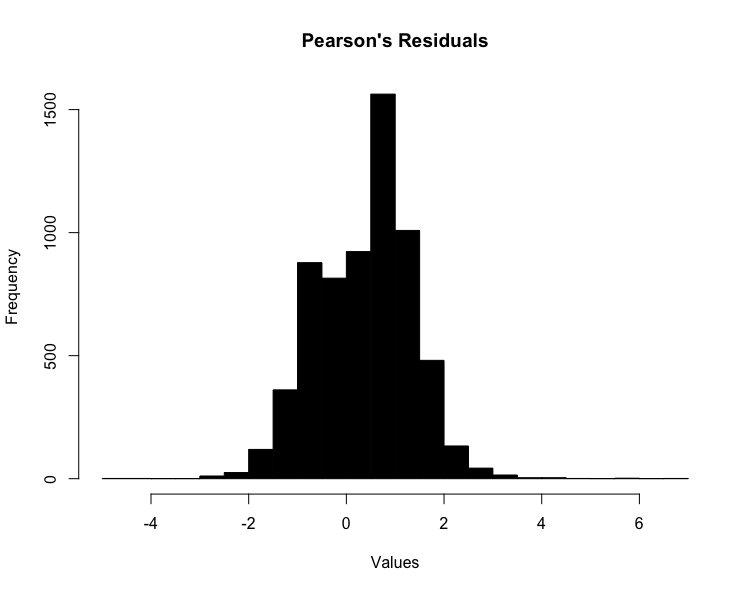
\includegraphics[width=.8\linewidth]{figures/pearson.png}
  \label{fig:sub1}
\end{subfigure}%
\begin{subfigure}{.5\textwidth}
  \centering
  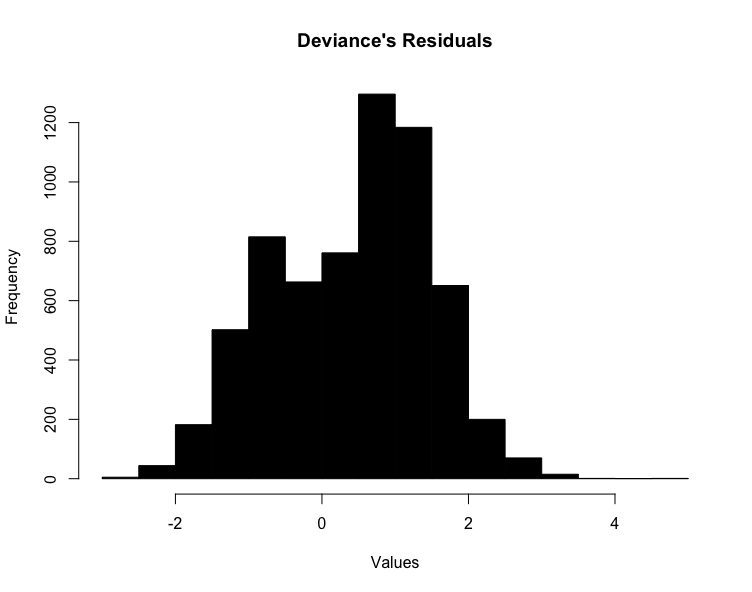
\includegraphics[width=.8\linewidth]{figures/deviance.png}
  \label{fig:sub2}
\end{subfigure}
\end{figure}

Both histograms look approximately normal, but the slight left skewness indicates potential for over-dispersion. The sum of squared residuals divided by degrees of freedom using Pearson's and Deviance residuals is 1.15 and 1.36, respectively, further indicating the presence of over-dispersion in our model.

One possible cause of over-dispersion is the effect of latent variables not specifically addressed by our model. We solve this problem in our next section by introducing a contest-specific predictor.

\subsection{Bradley-Terry Model with Contest-Specific Predictors}

The standard Bradley-Terry model above does not take any covariates into account. We offer a natural extension to the standard model, which adds an indicator if the team was playing at home or not. This addition results in the following logit representation:

$$\text{logit}[P(i \text{ beats } j)] = \alpha \times \mathbbm{1}_{\text{Team i is home}} + \beta_i - \beta_j$$

Here $\alpha$ is the 'Home Team Effect', or the increase in the Log-Odds of Team $i$ winning if they are playing at home.

\subsubsection{Results}

After running the model, the coefficient estimate for $\alpha$ is 0.546, with a Standard Error of 0.016. This estimate means that playing at home increases the odds of winning by a factor of $e^{0.546} = 1.726$. This result is quite significant, since, for example, a team with 2:1 normal odds would see their odds increase to almost 7:2 if playing at home. \textbf{INTERESTING! BECAUSE BOOKIES ONLY FAVOR HOME TEASM 53\%...WHY NOT MORE?? ARE WE SURE WE'RE INTERPRETING THIS CORRECTLY? I THINK SO BUT MAYBE JUST DOUBLE CHECK WITH THE NOTES? IF YOU WANT, YOU CAN INDICATE THAT BOOKIES ARE POTENTIALLY UNDER ESTIMATING THE EFFECT OF HOME FIELD ADVANTAGE!!}

As above, we present the model outcome for the 5 teams with the best and worst winning percentage:

\begin{table}[H]
\centering
\begin{tabular}{|r|rrrr|}
  \hline
 & Team Name & Win \% & $\hat{\lambda_i}$ & SE($\hat{\lambda_i}$) \\ 
  \hline
   &  FC Barcelona & 0.769 & 2.852 & 0.307 \\ 
 Best  &  Real Madrid CF & 0.750 & 2.447 & 0.287 \\ 
   &  SL Benfica & 0.745 & 3.162 & 0.510 \\ \cline{1-5}
   &  Cordoba CF & 0.079 & -1.584 & 0.673 \\ 
Worst   &  SpVgg Greuther Furth & 0.118 & -1.674  & 0.588 \\ 
   & FC Dordrecht & 0.118 & -2.537 & 0.601 \\
   \hline
\end{tabular}
\end{table}

Our $\hat{\lambda}$ estimates have changed, but still follow the same relative magnitude as before. We note that the same random matchup from before, depending on which team is home or not, changes:

\begin{table}[H]
\centering
\begin{tabular}{rrrrr}
  \hline
 & Team $i$ & Team $j$ & Win Percentage ($i$, $j$) & P[$i > j$] \\ 
  \hline
 & SL Benfica  & Standard de Liege & (0.75, 0.50) & 0.914 \\ 
   & Torino & LOSC Lille & (0.30, 0.48) & 0.138 \\ 
   & FC Nantes & SM Caen & (0.29, 0.29)  & 0.650 \\ 
   & FC Dordrecht & FC Porto & (0.12, 0.74) & 0.006 \\ 
   & Celtic & Reading & (0.72, 0.16) & 0.975 \\ 
   \hline
\end{tabular}
\end{table}

We see that the probability of winning significantly increases if we account for the 'Home Field Advantage'! \textbf{LOVE THIS}This result corroborates our original analysis and answers our question of whether playing at home offers a significant advantage.\\

\subsubsection{Model Comparison}

The estimate for over-dispersion in our current model using Pearson's and Deviance residuals is now 1.02 and 1.17, respectively. Adding the 'Home Team' contest-level predictor provides a better fit to the model than the standard one. This predictor may help explain variation in the data that the Teams-only model was not able to.\\

To test this finding, we perform an Analysis of Deviance test between our Standard Bradley-Terry model, and the current one with the added contest-level predictor. By adding the single predictor, the Residual Deviance decreases by 1125, and the Chi-Squared Test between the two models results in a p-value of $2.2e^{-16}$. This indicates that adding the extra degree of freedom is significant, so we conclude that the larger model fits the data better.

\subsection{Bradley-Terry Model with Team-Specific Predictors}
 
 The last question we seek an answer to is how important certain team-specific predictors are to predicting the outcome of a head-to-head matchup. We consider an extension of the model of the form:
 
 $$\lambda_i = \displaystyle\sum_{r=1}^{p} \beta_r x_{ir} + \epsilon_i$$

The ability of Team $i$ is related to explanatory variables $x_{i1},...,x_{ip}$, through a linear predictor with coefficients $\beta_{r}$ and independent errors $\epsilon_i$, with expected value of 0. Our Coefficient and Standard Error estimates of these team-specific variables are the following:\\

\begin{tabular}{rrr}
  \hline
 & $\hat{\beta}$ & SE($\hat{\beta}$)\\ 
  \hline
Play Speed  & -0.004 & -0.0009 \\
Play Passing  & -0.001 & 0.001 \\
Creation Passing  & 0.0007 & 0.001 \\
Creation Crossing  & 0.002 & -0.0009 \\
   \hline
\end{tabular}
\quad
\begin{tabular}{rrr}
  \hline
 & $\hat{\beta}$ & SE($\hat{\beta}$)\\ 
  \hline
Creation Shooting & -0.002 & 0.0012 \\
Defense Pressure  & 0.013 & 0.001 \\
Defense Aggression & 0.004 & 0.0009 \\
Defense Team Width  & -0.013 & 0.001 \\
   \hline
\end{tabular}\\
\\
\\
For example, if the score for 'Defense Pressure' increases by 10 points for a particular team, the odds of that team beating any other team increases by a factor of $e^{0.013} = 1.13$. Furthermore, if a team's score for 'Play Speed' increased by 10 points, their odds of defeating another team actually decreases by a factor of 0.33.\\

Defense Pressure, Aggression, and Team Width, when introduced to the model, decrease Deviance the most compared to the other variables. As a result, these variables are the most significant in this model in affecting the contest. This result is not surprising, as the famous sports adage goes, \textit{Defense Wins Championships}.\textbf{LOVE THIS}\\

Overall however, after running an ANOVA comparing team-level predictors with the previous 'Home Advantage' model results in a large p-value, suggesting that adding these team-specific effects does little to improve the model fit. We believe this result is due to the fact that the FIFA score is too subjective, as well as the fact that players move around teams too much for the scores to have much meaning. The one constant in each match is that one team is at home and one is away, which contributes significantly to the result. This simpler Home-Field model is also easier to interpret and communicate, so we move forward with it.

\subsection{Accuracy}

We assess the accuracy of our 'Home Advantage' model by training it on 70\% of the data and predicting match outcomes on the other 30\%. Diagnostics include an ROC Curve and Confusion Matrix.

\begin{figure}[H]
\centering
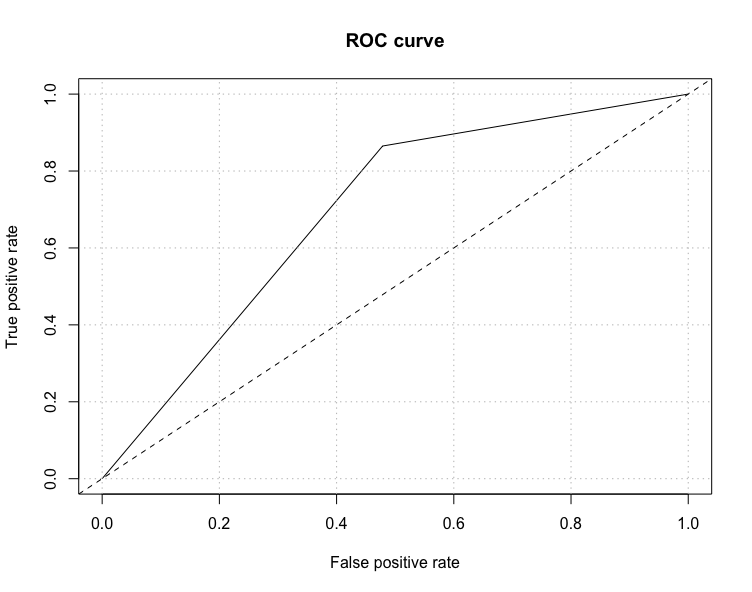
\includegraphics[width=.5\linewidth]{figures/roccurve.png}
\label{fig:sub1}
\end{figure}

\begin{table}[H]
\centering
\begin{tabular}{rrrrr}
  \hline
 & & Win &  Loss & Reference\\ 
  \hline
Prediction & Win  & 412 & 135 & \\
& Loss & 378 & 865 & \\
   \hline
\end{tabular}
\end{table}

\textbf{POSSIBLE TO GET THESE SIDE BY SIDE??}

We can see that the 'Home Advantage' model has a prediction accuracy of roughly 71\%. Furthermore, our AUC is 0.693, which is clearly better than random guessing and quite good given that our only external predictor is Home Field Advantage. \textbf{A LITTLE BIT CONCERNING THAT THE ROC CURVE ISN'T A "CURVE" BUT MORE OF TWO LINES. MAYBE DOUBLE CHECK QUICKKLY THAT THE CODE IS CORRECT? BUT DON'T SPEND MORE THAN 5 MINUTES ON IT.}

\section{Limitations and Further Extensions}

The key assumptions are in itself the limitations of the Bradley-Terry model for our analysis. The model assumes independent contests, which is unrealistic in a sports setting. Teams change throughout the season, and certain games will most definitely influence others. Another issue is that the Standard Bradley-Terry model removes all 'ties'. Davidson (1970) extended the B-T model to accommodate ties, and given that 25\% of the games in the dataset were ties, it would be very beneficial to explore this extension as to make full use of our dataset. \textbf{ADD IN THE PART FROM ABOVE SAYING THAT DIFFERENT TEAMS PLAY DIFFERENT TEAMS SO NOT CONSISTENT OPPONENTS?} Overall, however, the Bradley-Terry models are a robust, scalable, and interpretable method for modeling outcomes of competitions. They work particularly well for soccer matches, which have a clear win, loss, or tie, and their extensions add an interesting complexity.

\section{References}

[1] Agresti, Alan. Categorical Data Analysis. Hoboken, NJ: Wiley, 2013. Print.\\

[2] Borjigin, Khachin. "Players - FIFA 17 - Dec 1, 2016 - SoFIFA." Players - FIFA 17 - Dec 1, 2016 - SoFIFA. N.p., n.d. Web. 05 Dec. 2016.\\

[3] Bradley RA, Terry ME (1952). ?Rank Analysis of Incomplete Block Designs I: The Method
of Paired Comparisons.? Biometrika, 39, 324?45\\

[4] Davidson, Roger R. ?On Extending the Bradley-Terry Model to Accommodate Ties in Paired Comparison Experiments.? Journal of the American Statistical Association, vol. 65, no. 329, 1970, pp. 317?328. www.jstor.org/stable/2283595.\\

[5] Kaggle: Your Home for Data Science. N.p., n.d. Web. 05 Dec. 2016.\\

\end{document}

